% Digital Logic Report Template
% Created: 2020-01-10, John Miller

%==========================================================
%=========== Document Setup  ==============================

% Formatting defined by class file
\documentclass[11pt]{article}

% ---- Document formatting ----
\usepackage[margin=1in]{geometry}	% Narrower margins
\usepackage{booktabs}				% Nice formatting of tables
\usepackage{graphicx}				% Ability to include graphics

%\setlength\parindent{0pt}	% Do not indent first line of paragraphs 
\usepackage[parfill]{parskip}		% Line space b/w paragraphs
%	parfill option prevents last line of pgrph from being fully justified

% Parskip package adds too much space around titles, fix with this
\RequirePackage{titlesec}
\titlespacing\section{0pt}{8pt plus 4pt minus 2pt}{3pt plus 2pt minus 2pt}
\titlespacing\subsection{0pt}{4pt plus 4pt minus 2pt}{-2pt plus 2pt minus 2pt}
\titlespacing\subsubsection{0pt}{2pt plus 4pt minus 2pt}{-6pt plus 2pt minus 2pt}

% ---- Hyperlinks ----
\usepackage[colorlinks=true,urlcolor=blue]{hyperref}	% For URL's. Automatically links internal references.

% ---- Code listings ----
\usepackage{listings} 					% Nice code layout and inclusion
\usepackage[usenames,dvipsnames]{xcolor}	% Colors (needs to be defined before using colors)

% Define custom colors for listings
\definecolor{listinggray}{gray}{0.98}		% Listings background color
\definecolor{rulegray}{gray}{0.7}			% Listings rule/frame color

% Style for Verilog
\lstdefinestyle{Verilog}{
	language=Verilog,					% Verilog
	backgroundcolor=\color{listinggray},	% light gray background
	rulecolor=\color{blue}, 			% blue frame lines
	frame=tb,							% lines above & below
	linewidth=\columnwidth, 			% set line width
	basicstyle=\small\ttfamily,	% basic font style that is used for the code	
	breaklines=true, 					% allow breaking across columns/pages
	tabsize=3,							% set tab size
	commentstyle=\color{gray},	% comments in italic 
	stringstyle=\upshape,				% strings are printed in normal font
	showspaces=false,					% don't underscore spaces
}

% How to use: \Verilog[listing_options]{file}
\newcommand{\Verilog}[2][]{%
	\lstinputlisting[style=Verilog,#1]{#2}
}




%======================================================
%=========== Body  ====================================
\begin{document}

\title{ELC 2137 Lab 06: Seven Segment Decoder}
\author{Abigail Joseph}

\maketitle


\section*{Summary}

In this lab, we created a 7-segment decoder which displays 7-segment hex values on a Baysys3 board.   


\section*{Q\&A}

Q: List errors found in simulation. What does this tell you about why we run tests?\\
\\
A: When simulating, I got the value Z for all my outputs. Upon examination, when calling "ssegdecoder", I had assigned a value to the variable "num" other than the wire I had created in the test file. I didn't have any other errors, only because we did most of the programming all together. We run simulations so that small errors such as mine can be caught before everything is implemented on the hardware, where it takes much longer to identify errors and make and implement corrections.  \\
\\

Q: How many wires are connected to the 7-segment display? If the segments were not all connected together, how many wires would there have to be? Why do we prefer the current method vs. separating all of the segments? \\
\\
A: There are two 4-bit wires and one single bit wire coming into the display and one 2-bit wire, one 7-bit wire, and 3 single bit wires as outputs for a total of 8. If the segments were all separate wires, there would be 21 wires. The current method makes programming cleaner and less confusing; keeping track of assigning values to specific bits of 8 wires is a lot easier than trying to keep track of 21 wires.\\





\section*{Code}

\Verilog[firstline=23, caption=Mux ,label=code:file_1]{mux2_4b.sv}
\Verilog[firstline=23, caption=Mux Test ,label=code:file_2]{mux2_4b_test.sv}
\Verilog[firstline=23, caption=Sseg Decoder ,label=code:file_3]{sseg_decoder.sv}
\Verilog[firstline=23, caption=Sseg Decoder Test ,label=code:file_4]{sseg_decoder_test.sv}
\Verilog[firstline=23, caption=Sseg1 ,label=code:file_5]{sseg1.sv}
\Verilog[firstline=23, caption=Sseg1 Test ,label=code:file_6]{sseg1_test.sv}

\section*{Results}

\begin{figure}[ht] 
	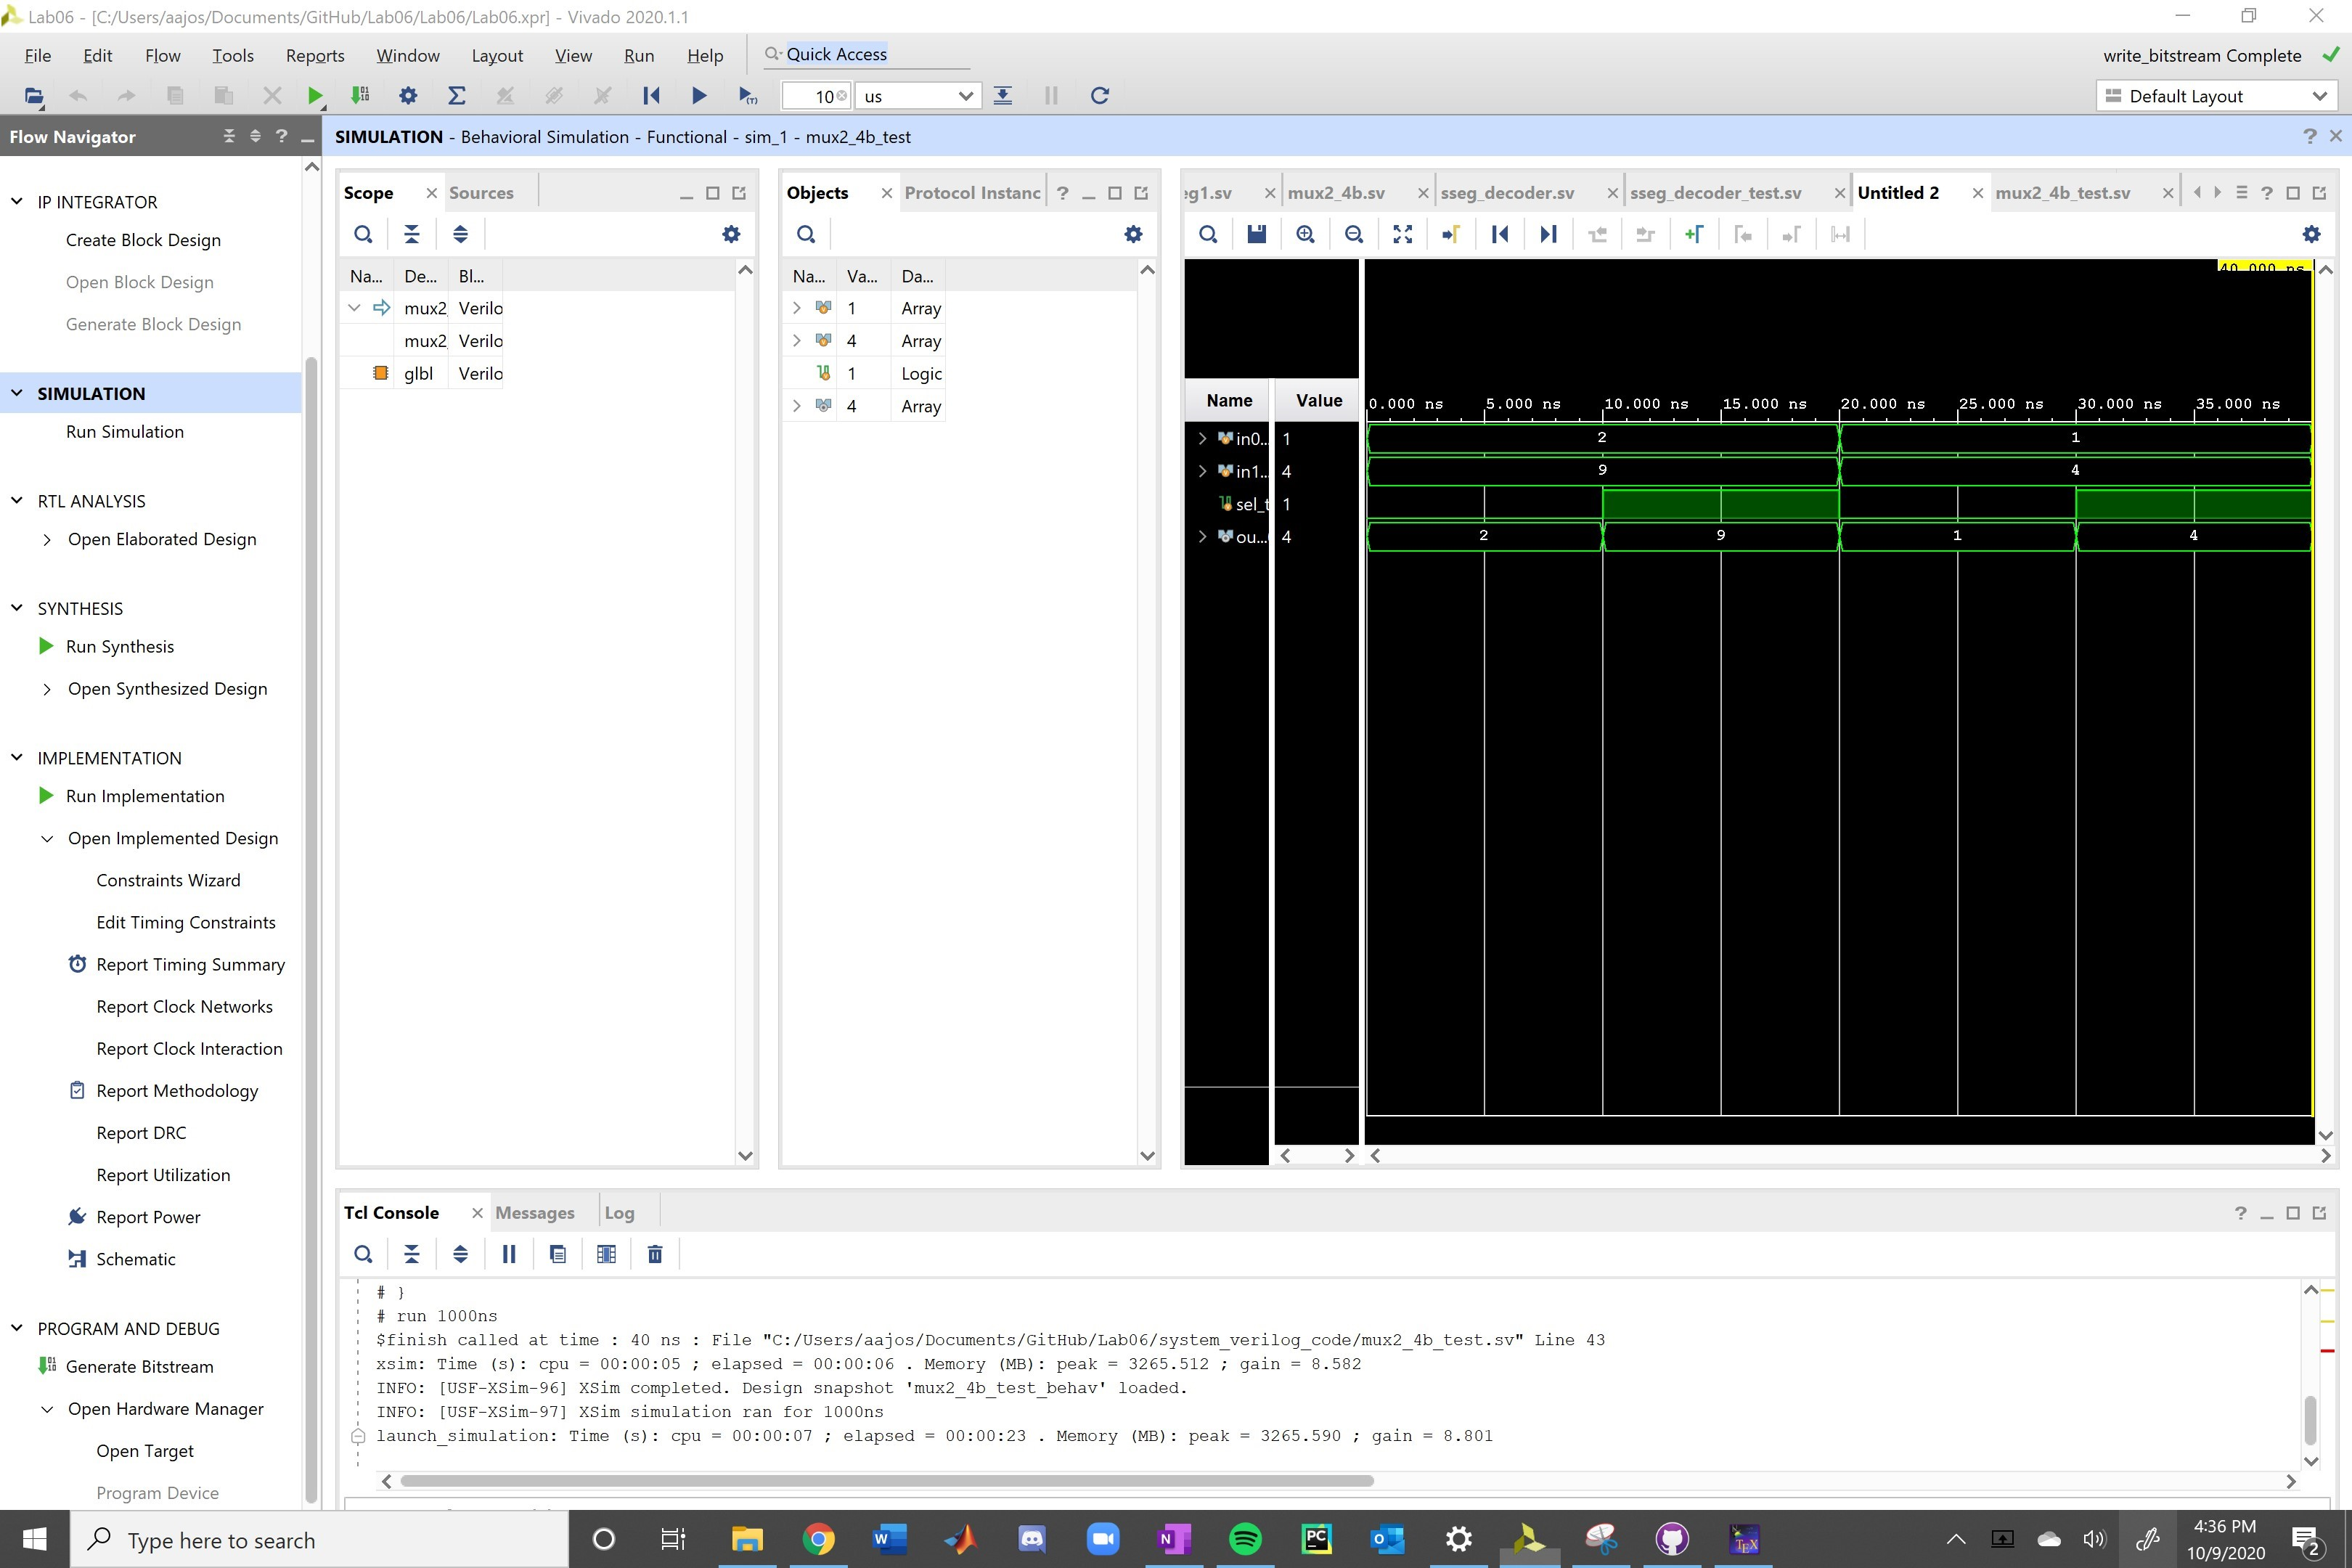
\includegraphics[width=1\textwidth,trim=19cm 14cm 0cm 6cm,clip]{mux2_4b_test_screen}
	\caption{Mux Test}
	\label{fig:mux2_4b_scrn}
\end{figure}


\begin{figure}[ht]
	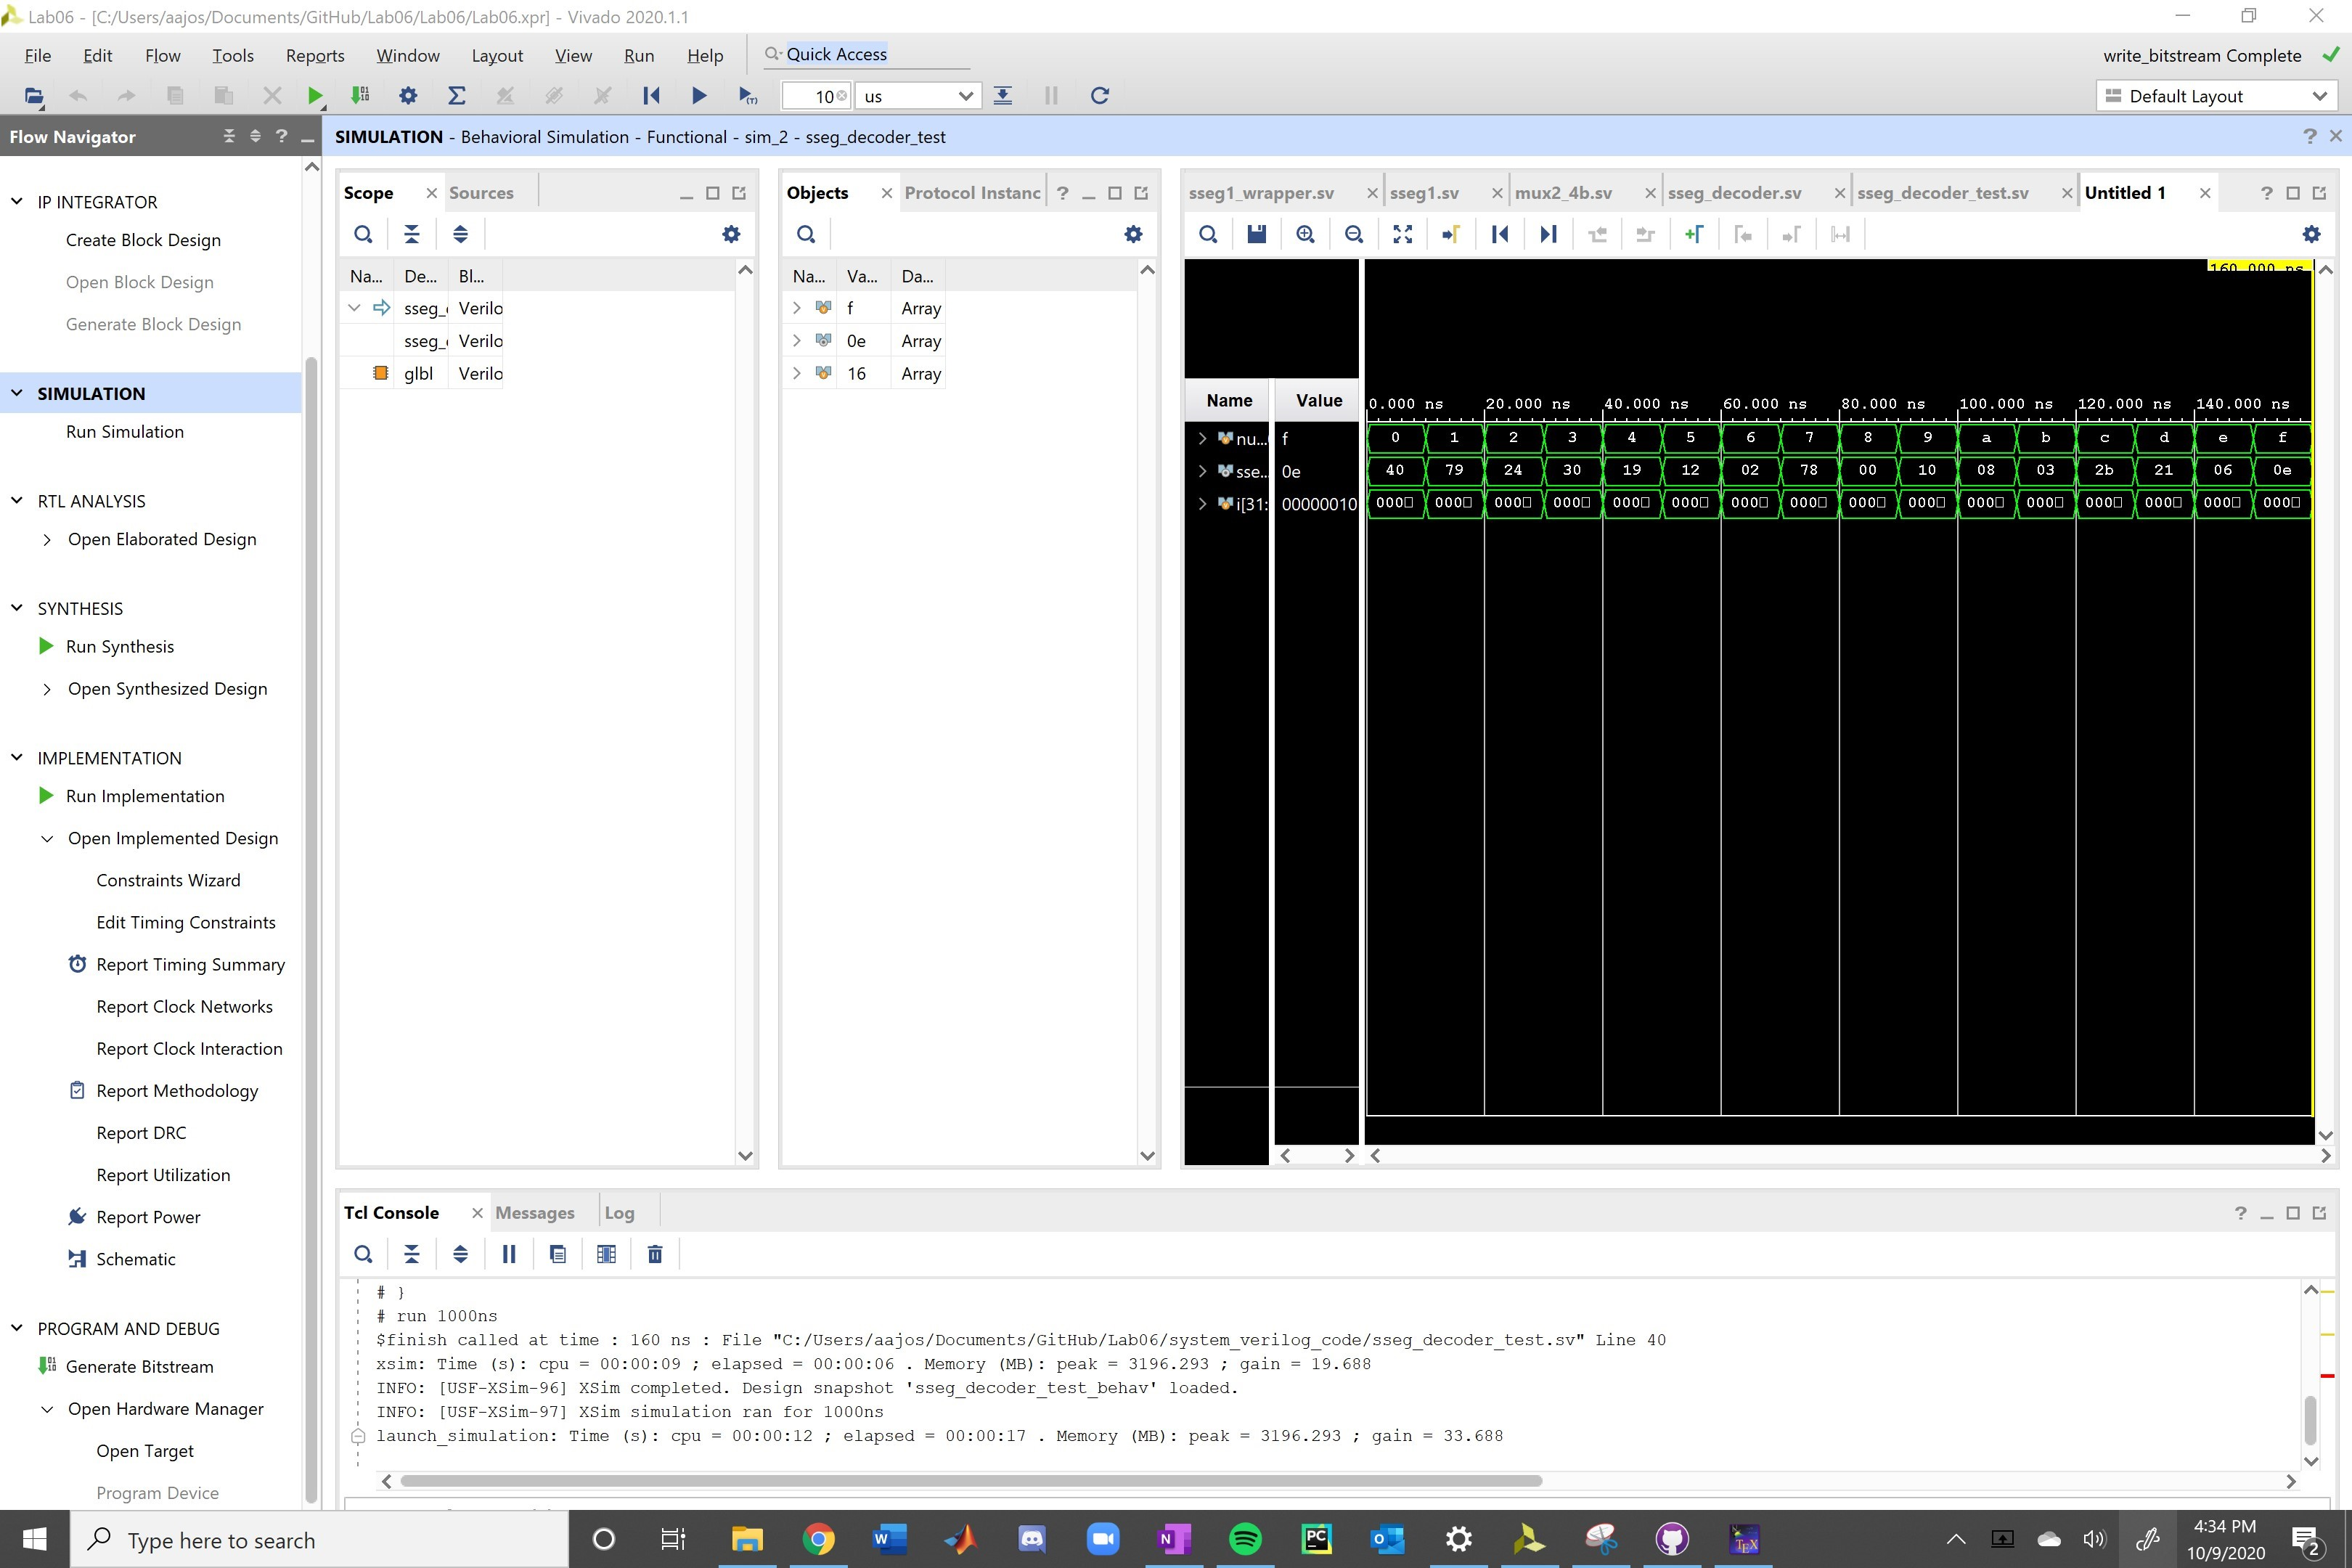
\includegraphics[width=1\textwidth,trim=19cm 14cm 0cm 6cm,clip]{sseg_decoder_test_screen}
	\caption{Sseg Decoder Test}
	\label{fig:sseg_decoder_scrn}
\end{figure}

\begin{figure}[ht]
	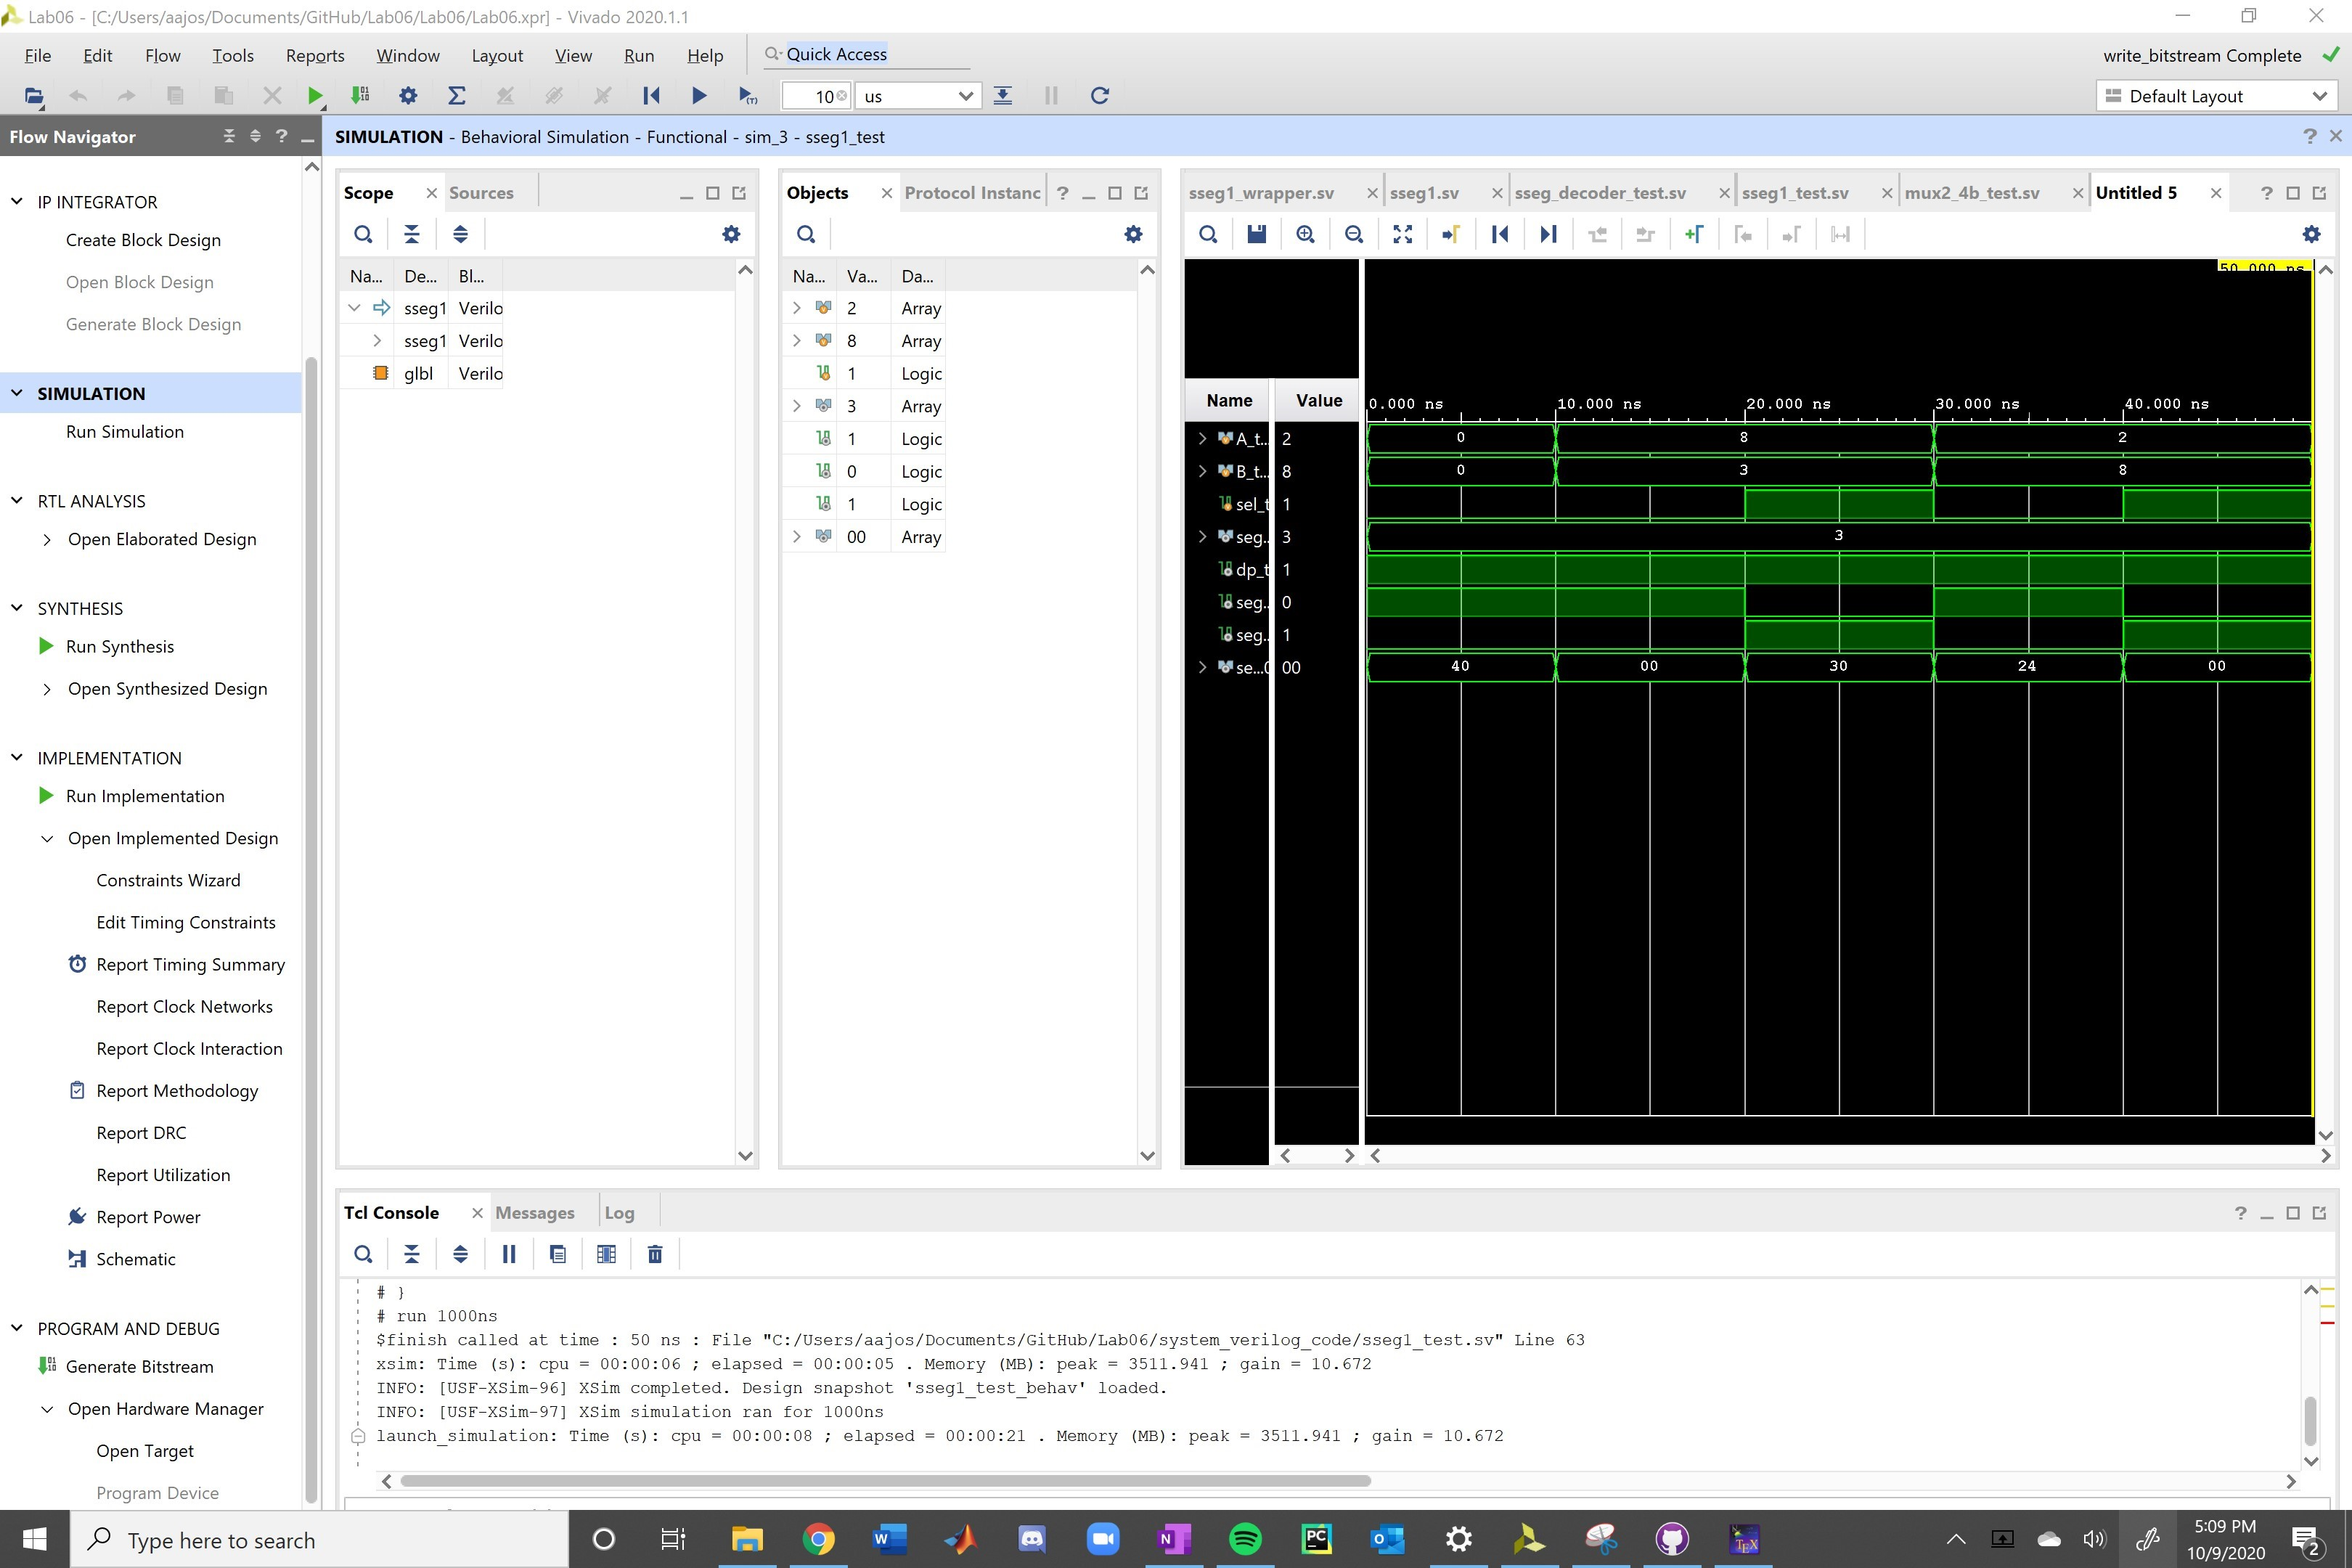
\includegraphics[width=1\textwidth,trim=19cm 14cm 0cm 6cm,clip]{sseg1_test_screen}
	\caption{Sseg1 Test}
	\label{fig:sse1g_scrn}
\end{figure}

\begin{figure}[ht]\centering
	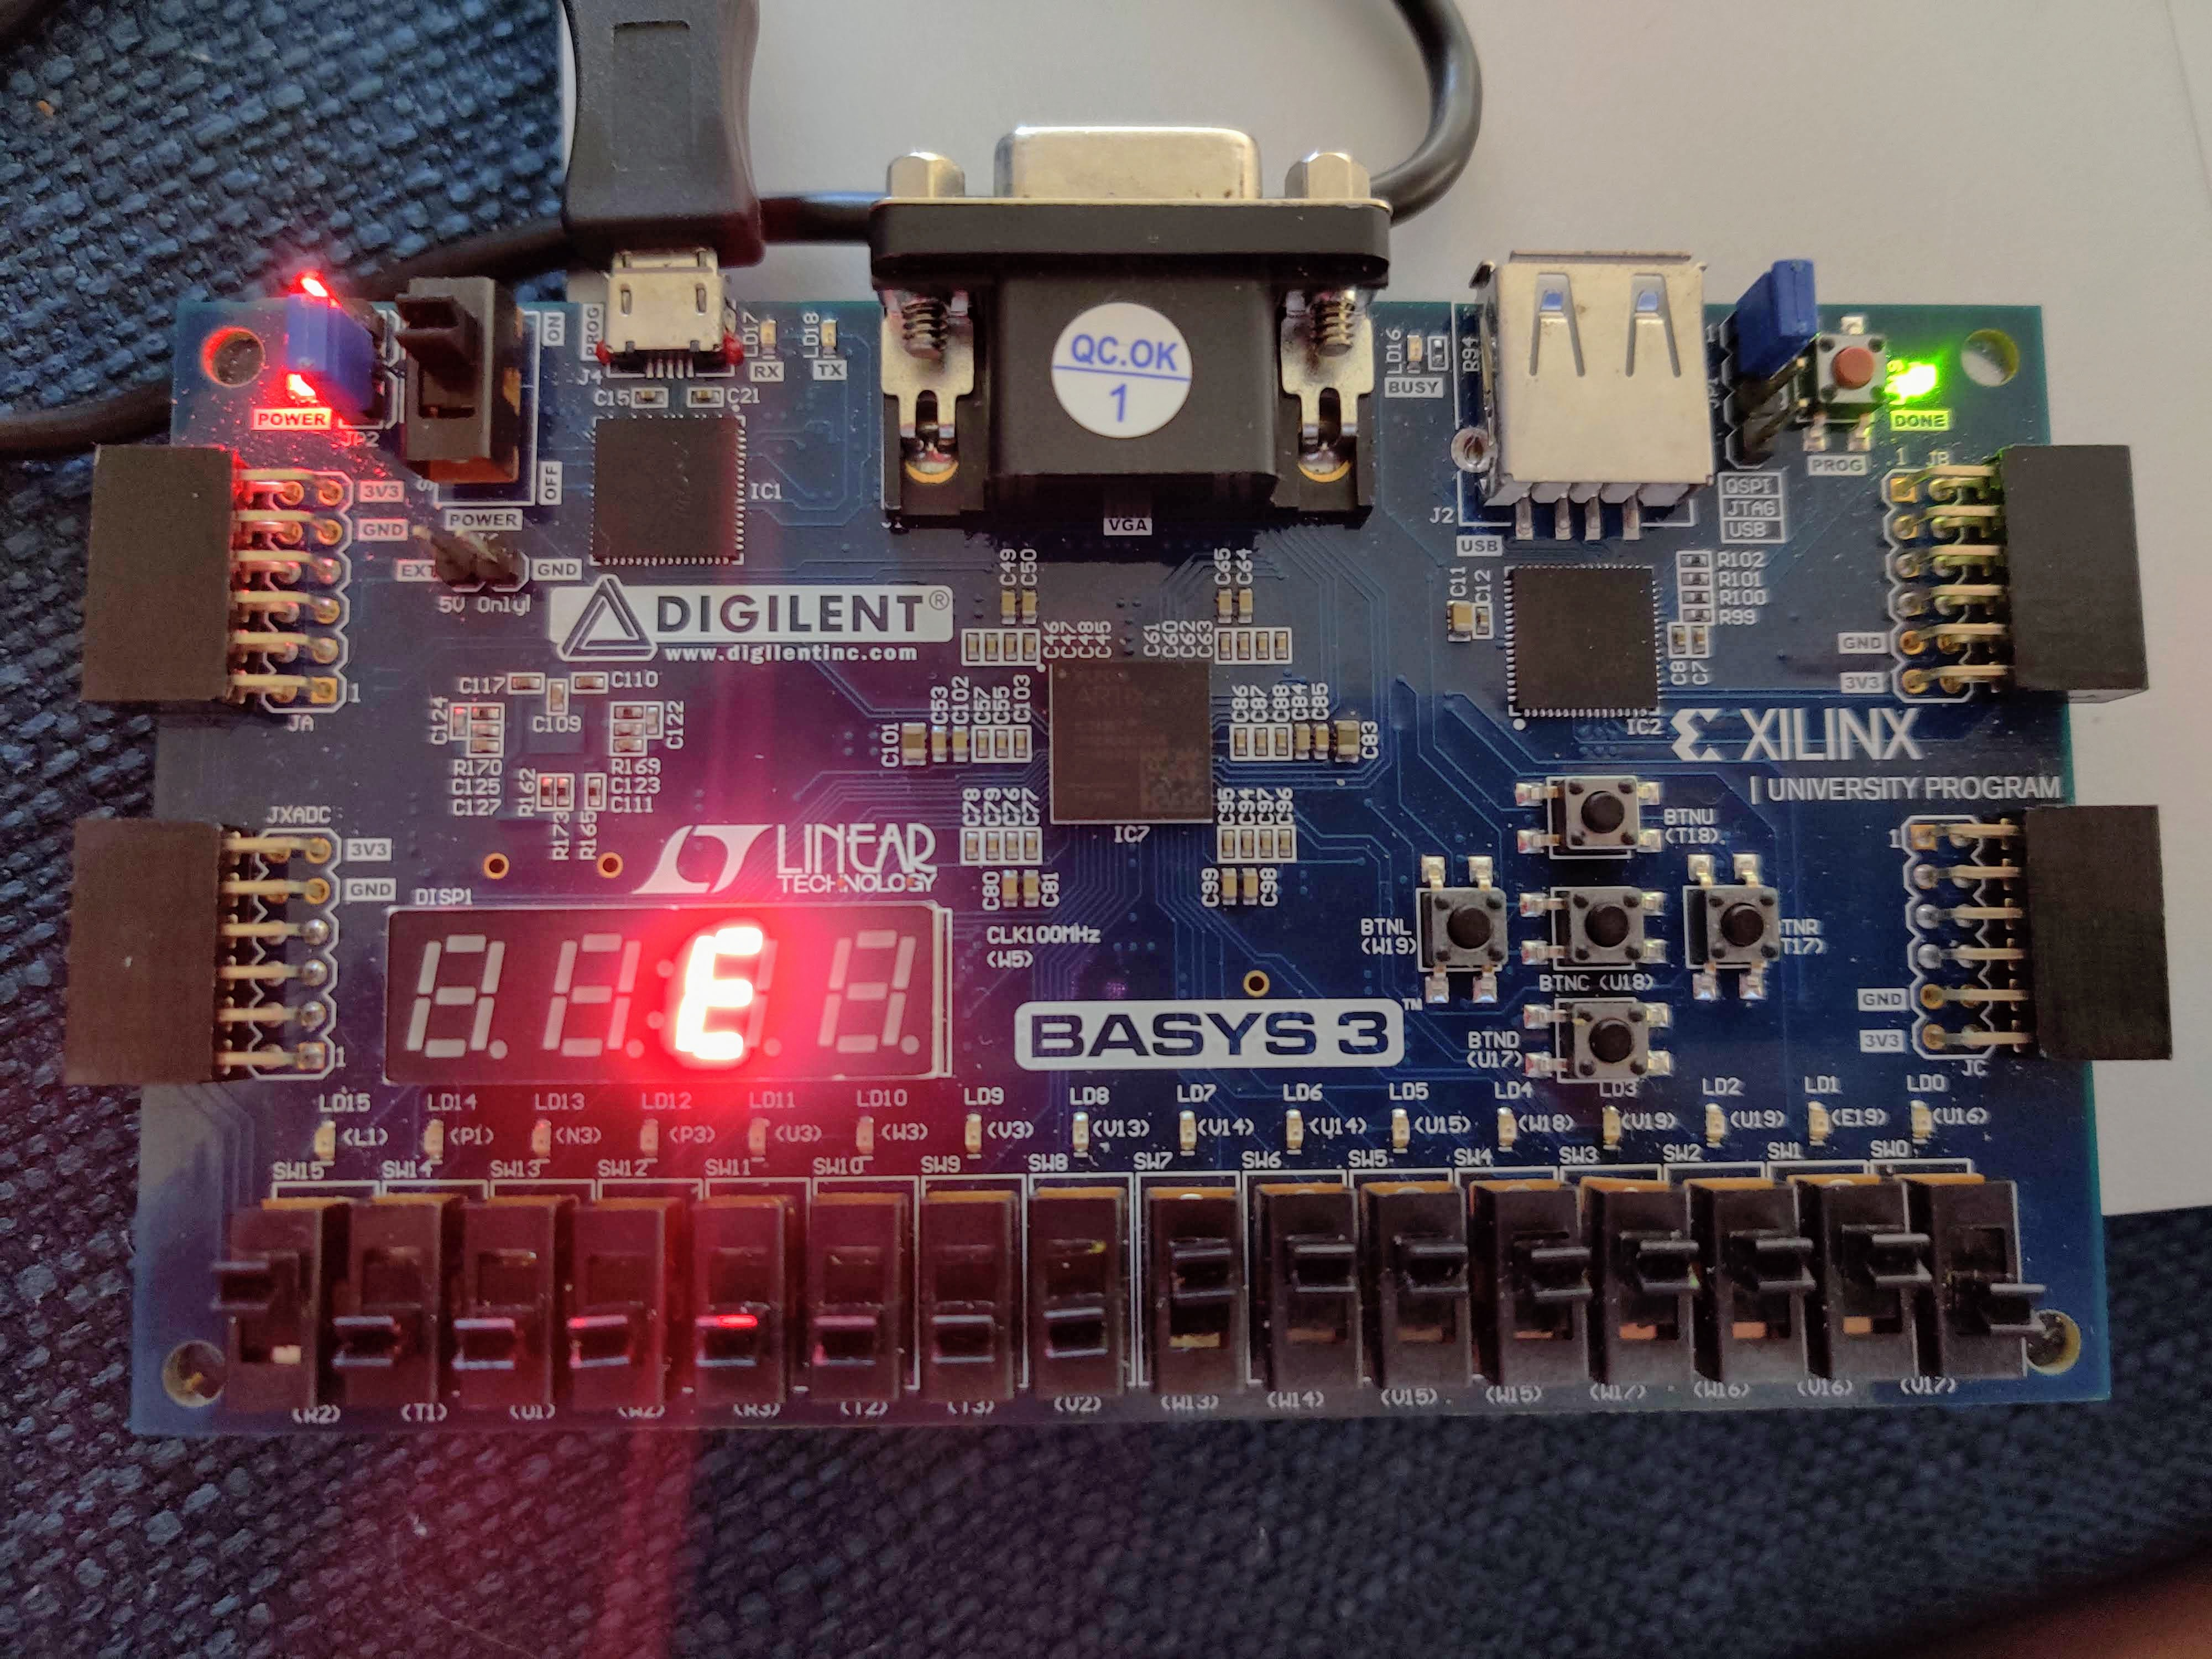
\includegraphics[width=.5\textwidth]{basys3_lab06_1}
	\caption{Basys 3 01}
	\label{fig:b3_0}			
\end{figure}

\begin{figure}[ht]\centering
	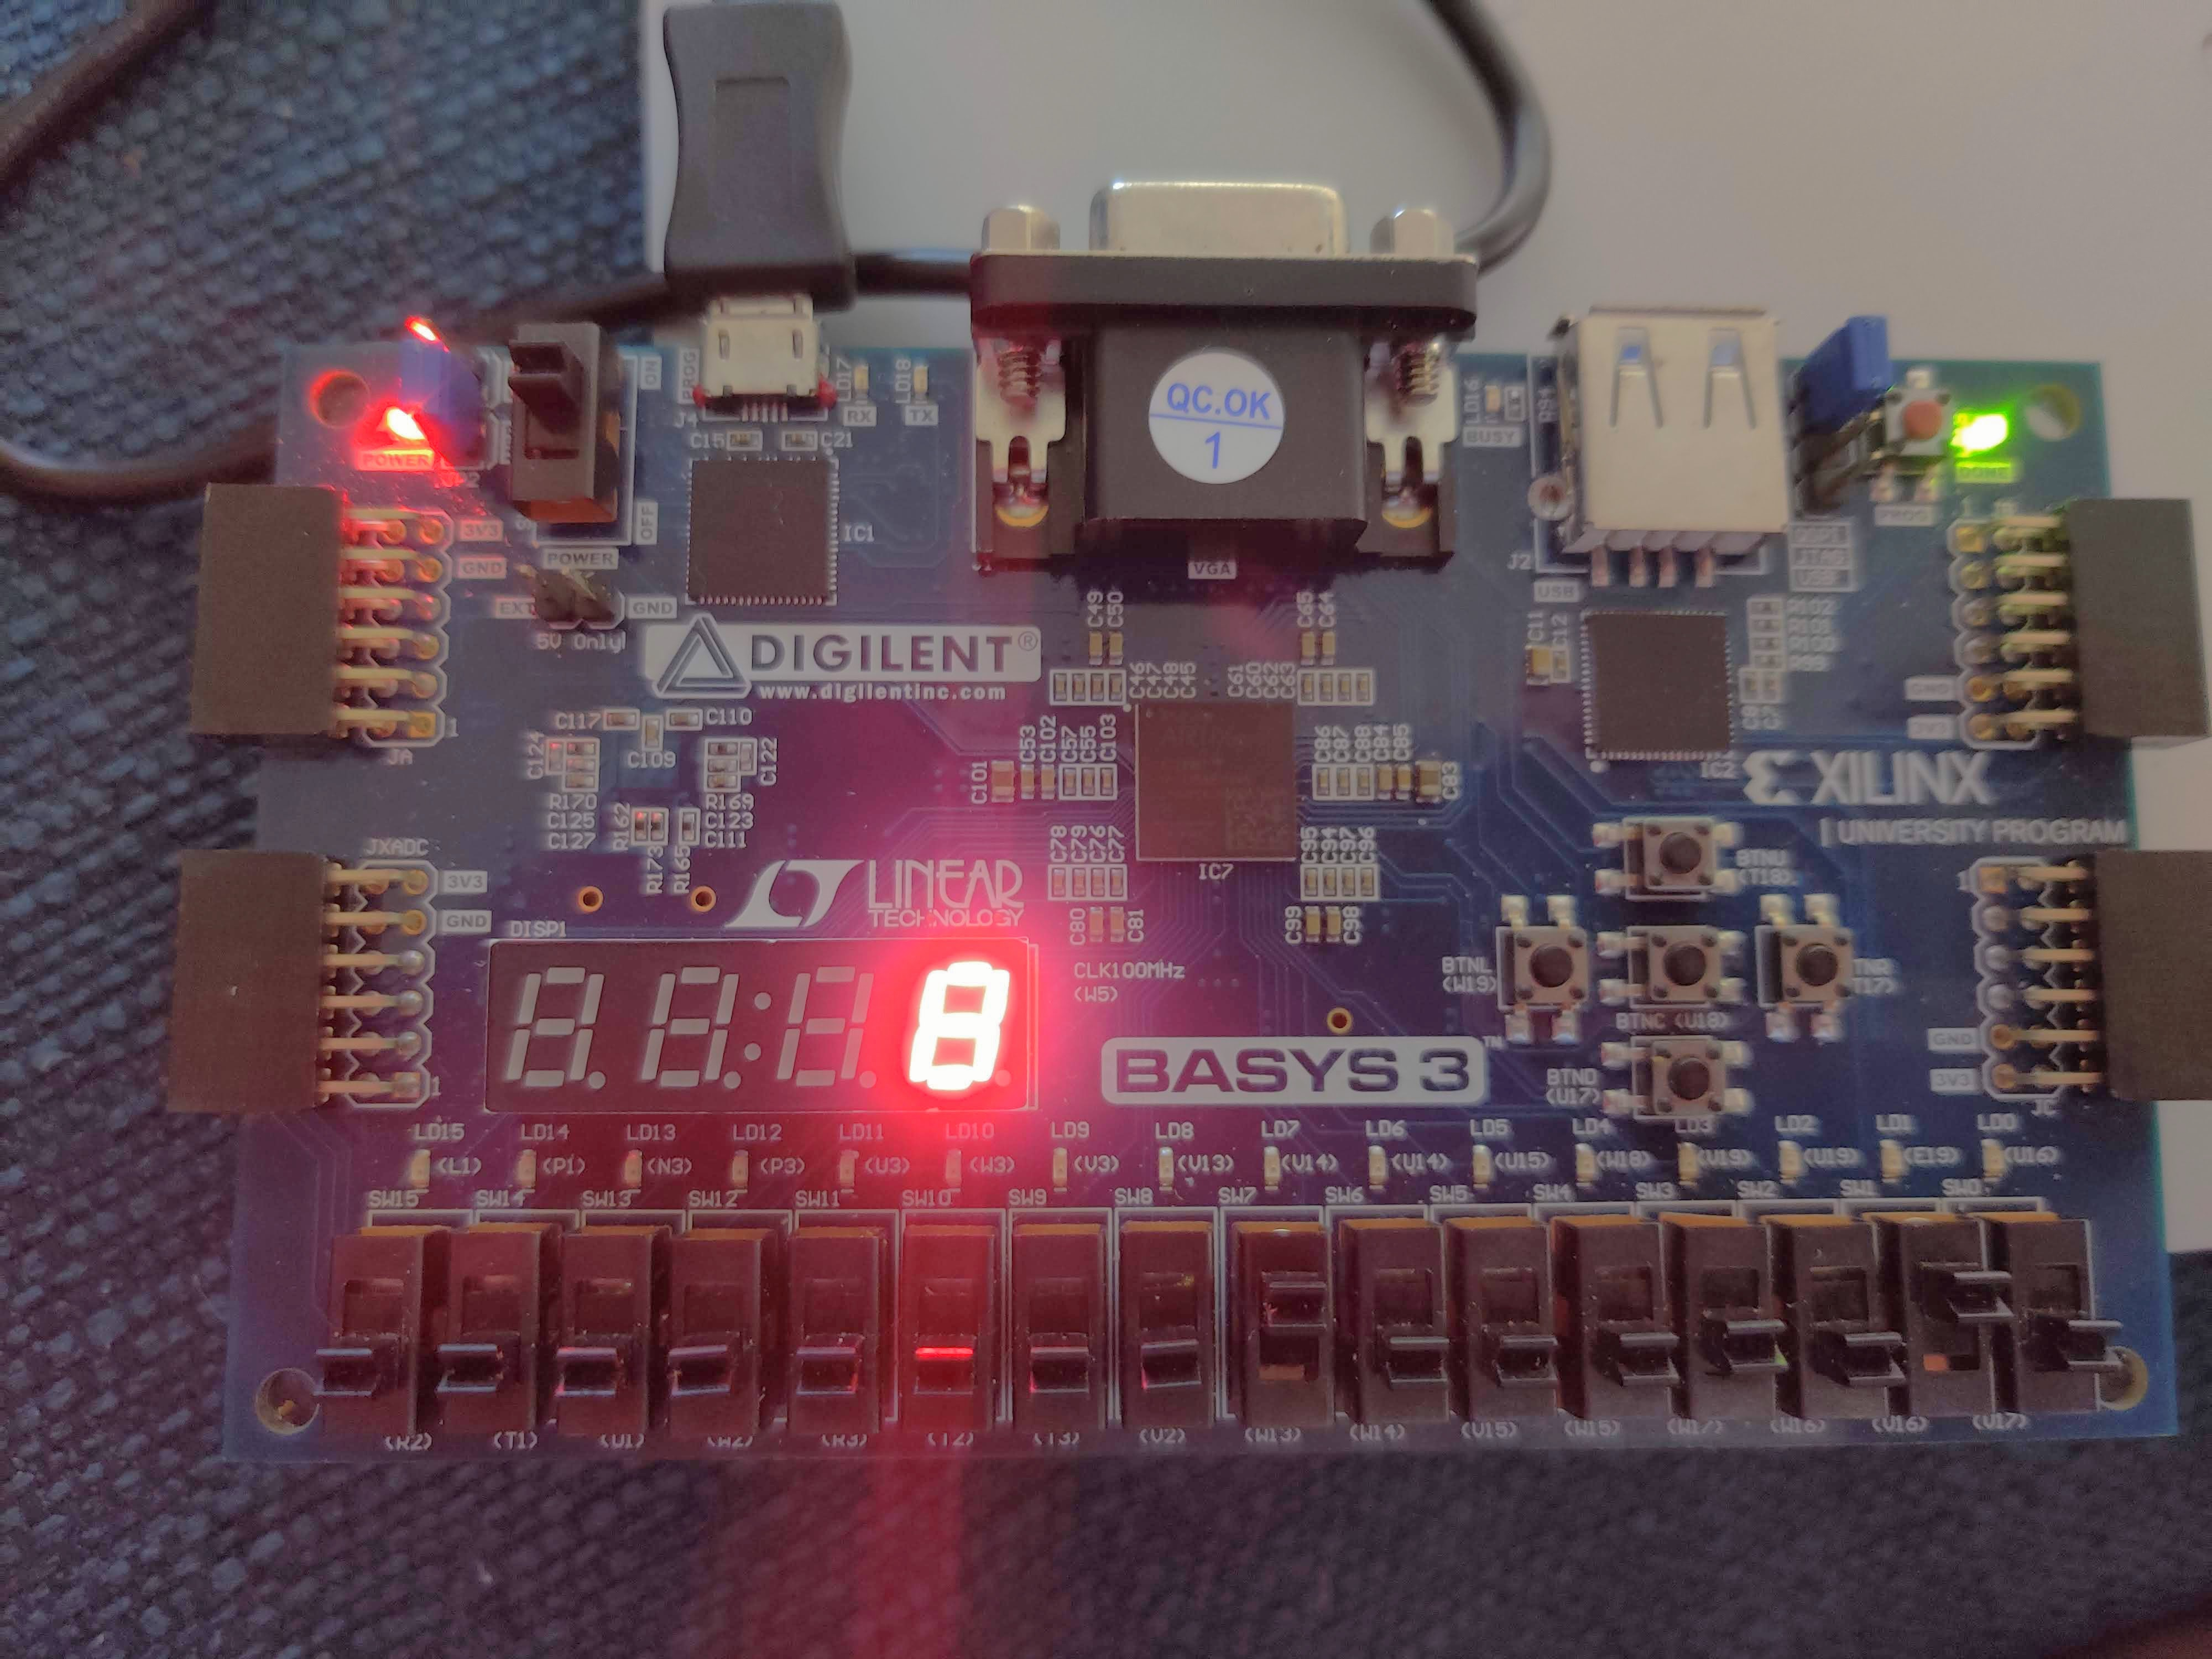
\includegraphics[width=.5\textwidth]{basys3_lab06_0}
	\caption{Basys 3 02}
	\label{fig:b3_1}			
\end{figure}

\end{document}
